\newpage

\begin{remark} Дополнение к предыдущей лекции: исправление доказательства достаточности критерия Лебега (в файле, присланном Александром Ивановичем, всё правильно)

Сначала вспомним, что было на прошлой лекции:

$C[f]$ -- м-во всех т. непрерывности ф-ии $f$

$\D[f]$ -- м-во всех т. разрыва $f$

$\bigcup_{i=1}^{\infty}(a_i, b_i) \supset \D[f]$
\hfill
$\sum_{i=1}^{\infty} |b_i - a_i| < \frac{\epsilon}{2M}$

$\forall x \in C[f]\quad \exists I(x):\; \omega_{3I(x)}f < \frac{\epsilon}{b - a}$

$\left(\bigcup_{x\in C[f]} I(x)\right) \cup \left(\bigcup_{i=1}^{\infty}(a_i,b_i)\right)$ -- покрытие отрезка $[a, b]$

Выберем конечное подпокрытие $\{(c_j, d_j)\}_{j=1}^L$ -- конечное подпокрытие

Разобьём интервалы на хорошие и плохие. Хорошими назовём интервалы из первого семейства, из $\bigcup_{x\in C[f]} I(x)$, то есть те, которые покрывают точки непрерывности. Плохими назовём интервалы из второго семейства $\bigcup_{i=1}^{\infty}(a_i,b_i)$

$T = \{x_i\}_{i=0}^{N_T}$ -- разбиение отрезка $[a, b]$

Место, где была ошибка:

$[x_{i-1}, x_i]$ назовём хорошим, если он пересекает хороший интервал (на прошлой лекции было сказано, что если он пересекает множество точек непрерывности)

В противном случае назовём отрезок плохим

Дальше всё верно
\end{remark}

\subsubsection{Следствия из критерия Лебега}
\begin{enumerate}
    \item Если $f \in R([a, b])\text{, то } f\in R([a', b'])\quad \forall a \leqslant a' \leqslant b' \leqslant b$
    \begin{proof}
        \begin{enumerate}
            \item $\B([a, b]) \subset \B([a', b'])$
            \item $\D[f] \cap [a', b'] \subset \D[f]\cap [a, b]$
            но $\forall$ подмножество множества лебеговой меры 0 само имеет лебегову меру 0
            Отсюда по критерию Лебега получается искомое
        \end{enumerate}
    \end{proof}
    \item Если $f \in R([a, b]), g\in R([a, b]) \implies fg \in R([a, b])$
    \begin{proof}
    \begin{enumerate}
        \item $g, f \in \B([a, b]) \implies f\cdot g \in \B([a, b])$

        \item Если $f$ непрерывна в т. $x^0 \in [a, b]$ и $g$ непрерывна в т. $x^0\in [a, b] \implies f\cdot g$ непрерывна в т. $x^0 \in [a, b]$

        $C[f] \cap C[g] \subset C[fg]$

        $\implies \D[gf] \subset \D[f] \cup \D[g]$

        Другими словами, $[a, b] \setminus (G_1 \cap G_2) = [a, b] \setminus G_1 \cup [a, b] \setminus G_2$

        $\D[f]\text{ и }\D[g]$ имеют лебегову меру 0, значит $\D[gf]$ имеет лебегову меру 0
    \end{enumerate}
    $\implies$ в силу критерия Лебега имеем искомое
    \end{proof}
\end{enumerate}

\begin{reminder}
    \begin{definition}
        Ф-ия $f \in R([a, b]) \Longleftrightarrow$
        
        $\exists J \in \R:\; \forall \epsilon > 0\; \exists \delta(\epsilon):\; \forall T: \; l(T) < \delta \hookrightarrow |s(f, T) - J| < \epsilon,\; |S(f, T) - J| < \epsilon$
    \end{definition}\bigskip
    
     \textbf{Критерий в терминах интегральных сумм Римана}
    
     $f \in R([a, b]) \Longleftrightarrow \exists J: \forall \epsilon > 0\; \exists \delta(\epsilon): \forall T \text{ -- разбиение }[a, b]: l(T) < \delta(\epsilon)\text{ и }\forall\xi_T\text{ -- выборки,}$
     
     $\text{соответстующей разбиению } T\quad \hookrightarrow |\Sigma(f, T, \xi_T) - J|< \epsilon$
     
     Этот критерий можно ''вульгарно''\; записать как: $\lim_{l(T)\rightarrow 0}\Sigma(f, T, \xi_T) = J$.
     Договоримся, что эта запись означает кванторное выражение, записанное выше.
     
     
     $\int_a^b f(x)dx := J$ -- это число $J$ и есть определённый интеграл Римана

     Конец напоминания
\end{reminder}

Интегральные суммы Римана полезны для доказательства последующего утверждения\bigskip

Мы пока не говорили, какая структура у множества всех интегрируемых на $[a, b]$ функций, а на самом деле это линейное пространство. Давайте это докажем

\begin{theorem}
    Пусть $f, g \in R([a, b])$. Тогда $\forall \alpha, \beta$

    $\alpha f + \beta g \in R([a, b])$ и, кроме того,

    $\int_a^b (\alpha f(x) + \beta g(x)) dx = \alpha \int_a^b f(x)dx + \beta \int_a^b g(x)dx$
\end{theorem}
\begin{proof}
    $\forall T$ - разб. о-ка $[a, b] \forall$ выборки $\xi_T$ соответств. разбиению $T$

    \begin{equation}
    \Sigma(\alpha f + \beta g, T, \xi_T) = \alpha \Sigma(f, T, \xi_T) + \beta \Sigma(g, T, \xi_T) \label{eq:int_lin_proof}
    \end{equation}

    Переходя к пределу в этом равенстве при мелкости разбиения стремящейся к 0, получим искомое\bigskip

    Распишем этот переход подробнее:

    Фиксируем $\epsilon > 0$ и, пользуясь тем, что $f, g \in R([a, b])$,
    найдём $\delta(\epsilon) > 0:\; \forall T\text{ -- разб. о-ка }[a, b]$
    
    $\text{ и } \xi_T\text{ -- выборки  }$ 

    $|\Sigma(f, T, \xi_T) - \int_a^b f(x)dx| < \epsilon$

    $|\Sigma(g, T, \xi_T) - \int_a^b g(x)dx| < \epsilon$

    Но тогда в силу \eqref{eq:int_lin_proof}

    $|\Sigma (\alpha f + \beta g, T, \xi_T) - \alpha \int_a^b f(x)dx - \beta \int_a^b g(x)dx| \leqslant \alpha |\Sigma(f, T, \xi_T) - \int_a^b f(x)dx| + \beta|\Sigma(g, T, \xi_T) - \int_a^b g(x)dx \leqslant \alpha \epsilon + \beta \epsilon$

    Но $\epsilon > 0$ выбрано произвольно $\implies$ пользуясь критерием в терминах интегральных сумм Римана, получаем искомое
\end{proof}

\begin{theorem}
    \textbf{Интегрирование неравенств.}
    Пусть $f, g \in R([a, b])$ и $f(x) \leqslant g(x)\quad \forall x \in [a, b]$.
    Тогда $\int_a^b f(x)dx \leqslant \int_a^b g(x)dx$ 
\end{theorem}
\begin{proof}
    $\forall T$ -- разбиения о-ка $[a, b]$ и $\forall\xi_T$ -- выборки соответствующей разбиению $T$

    $\Sigma(f, T, \xi_T) \leqslant \Sigma(g, T, \xi_T)$

    Переходя к пределу в неравенстве, аналогично предыдущей теореме, и пользуясь критерием в терминах интегральных сумм Римана, получаем искомое
\end{proof}
\begin{theorem}
    \textbf{Интегрируемость модуля.} Если $f \in R([a, b])$, то $|f| \in R([a, b])$ и справедливо неравенство

    \begin{equation}
        \left|\int_a^b f(x)dx\right| \leqslant \int_a^b |f(x)|dx
        \label{eq:int_of_abs}
    \end{equation}
\end{theorem}
\begin{proof}
    Пусть $f \in R([a, b]) \implies$ по критерию Лебега $f \in B([a, b])$
    и $\D[f]$ имеет лебегову меру 0.

    $\implies |f| \in B([a, b])$.

    Если $f$ непрерывна в т. $x^0 \in [a, b]$, то $|f|$ тоже непрерывен
    в этой точке $x^0$.

    $\D[|f|] \subset \D[f]$, а так как $\D[f]$ имеет лебегову меру 0,
    $\D[|f|]$ тоже имеет лебегову меру 0

    $\implies$ в силу критерия Лебега \underline{$|f| \in R([a, b])$}

    Теперь докажем \eqref{eq:int_of_abs}.
    $\left\{\begin{aligned}
        f(x) \leqslant |f(x)|\quad \forall x \in [a, b] \\
        -f(x) \leqslant |f(x)| \quad \forall x \in [a, b]
    \end{aligned}\right.$

    $\implies$ в силу т. об интегрировании неравенств

    \[ \left\{ \begin{aligned}
    \int_a^b f(x)dx \leqslant \int_a^b |f(x)| dx \\
    \int_a^b -f(x)dx \leqslant \int_a^b |f(x)|dx
    \end{aligned} \right. \]

    Воспользуемся предпредыдущей теоремой про линейную комбинацию, при $\alpha = -1, \beta = 0$: $\int_a^b -f(x)dx = -\int_a^b f(x)dx$

    \[ \left\{ \begin{aligned}
    \int_a^b f(x)dx \leqslant \int_a^b |f(x)| dx \\
    \int_a^b f(x)dx \geqslant -\int_a^b |f(x)|dx
    \end{aligned} \right. \]

    $\left|\int_a^b f(x)dx\right| \leqslant \int_a^b |f(x)|dx$
\end{proof}

\begin{theorem}
    \textbf{Аддитивность интеграла по отрезкам.}
    Пусть $f\in \Rim([a, b])$ и $f \in \Rim([b, c])$, где $a \leqslant b \leqslant c$.
    
    Тогда $f \in R([a, c])$ и справедливо равенство 

    $\int_a^c f(x)dx = \int_a^b f(x)dx + \int_b^c f(x)dx$
\end{theorem}
\begin{proof}
    Пусть $T = \{x_i\}_{i = 0}^{N_T}$ -- разбиение $[a, c]$.
    Пусть $j \in \{0, \hdots, N_T\}:\; b \in [x_{j - 1}, x_j]$

    $T_1 = \{x_i\}_{i = 0}^{j - 1} \cup \{b\}$ -- разбиение о-ка $[a, b]$

    $T_2 = \{b\}\cup\{x_i\}_{i = j}^{N_T}$ -- разбиение о-ка $[b, c]$
    
    Если $l(T) < \delta(\epsilon) \implies \begin{cases}
        \begin{aligned}    
    l(T_1) & \leqslant l(T) < \delta(\epsilon) \\
    l(T_2) & \leqslant l(T) < \delta(\epsilon)
    \end{aligned}
    \end{cases}$

    Т.к. $f \in R([a, b])$ и $f \in R([b, c]) \implies f \in B([a, b])$ и
    $f \in B([b, c])$

    $\implies f \in B([a, c]) \implies \exists M \geqslant 0:\;
    |f(x)| \leqslant M \quad \forall x \in [a, c]$

    Рассмотрим $S(f, T) - S(f, T_1) - S(f, T_2)$

    $S(f, T) = \sum_{i = 1}^{N_T}{M_i(x_i - x_{i - 1})}$
    
    $S(f, T_1) = \sum_{i = 1}^{j-1}{M_i(x_i - x_{i - 1})}
    + \left(\sup_{x \in [x_{j - 1}, b]} f(x) \right) \cdot (b - x_{j-1})$

    $S(f, T_2) = \sum_{i = j}^{N_T}{M_i(x_i - x_{i - 1})}
    + \left(\sup_{x \in [b, x_j]} f(x) \right) \cdot (x_j - b)$

    $|S(f, T) - S(f, T_1) - S(f, T_2)| \leqslant \left|M_j(x_j - x_{j-1}) - (b - x_{j - 1})\sup_{x\in[x_{j-1}, b]}f(x) - (x_j - b)\sup_{x\in[b, x_j]}f(x)\right| \leqslant \\
    \leqslant |M_j|(x_j - x_{j-1}) + (b - x_{j-1})|M_j| + (x_j - b)|M_j|
    \leqslant 2M(x_j - x_{j-1})
    \leqslant 2M l(T)$\bigskip

    $\implies \exists \lim_{l(T) \rightarrow 0} S(f, T) = \lim_{l(T_1) \rightarrow 0} S(f, T_1) + \lim_{l(T_2) \rightarrow 0} S(f, T_2) = \int_a^b f(x)dx + \int_b^c f(x)dx$

    Аналогично для нижних сумм Дарбу, и тогда по определению
    интегрируемости ч. т. д.
\end{proof}\bigskip\bigskip

\textbf{Соглашение.}
Договоримся, что если $a < b$

$\int_b^a f(x)dx := -\int_a^b f(x)dx$

\begin{corollary}
    При любом расположении точек $a, b, c$, если $f$
    интегрируема на отрезке, содержащем $a, b, c$, то
    $\int_a^c f(x) dx = \int_a^b f(x)dx + \int_b^c f(x)dx$
\end{corollary}

\subsubsection{Связь определённого и неопределённого интеграла}
\begin{definition}
    Будем говорить, что $F$ -- первообразная ф-ии $f$ на о-ке $[a, b]$

    $-\infty < a < b < +\infty$, если 

    \begin{equation*} \begin{cases}    
        F'(x) = f(x) \quad \forall x \in (a, b) \\
        F'_+(a) = f(a) \\
        F'_-(b) = f(b)
    \end{cases} \end{equation*}
\end{definition}

\begin{remark}
    Множество всех функций, имеющих первообразную на $[a, b]$,
    и множество всех функций, интегрируемых по Риману на $[a, b]$,
    пересекаются, но ни одно из них не является подмножеством другого

    Обозначим множество всех функций, имеющих первообразную на $[a, b]$, но неинтегрируемых по Риману на $[a, b]$, за (1)

    Множество всех функций, интегрируемых по Риману на $[a, b]$, но не имеющих первообразную на $[a, b]$, обозначим за (2)

    А множество всех функций, имеющих первообразную на $[a, b]$ и интегрируемых по Риману на $[a, b]$, обозначим за (3)
\end{remark}

Приведём пример функции из множества (1)

Рассмотрим следующую функцию:

\begin{equation}
F(x) = \begin{cases}
    x^2\cdot \sin \frac{1}{x^2}, & x \neq 0 \\
    0, & x = 0
\end{cases}
\label{eq:for_not_Reimann_integrable}
\end{equation}

КАРТИНОЧКА
% {
%     \input{Pictures|Fancy_sinus_for_not_Riemann_integrable_example.png}
% }
% \caption{График функции \eqref{eq:for_not_Reimann_integrable}}

% \begin{wrapfigure}{R}{0.4\textwidth}
% 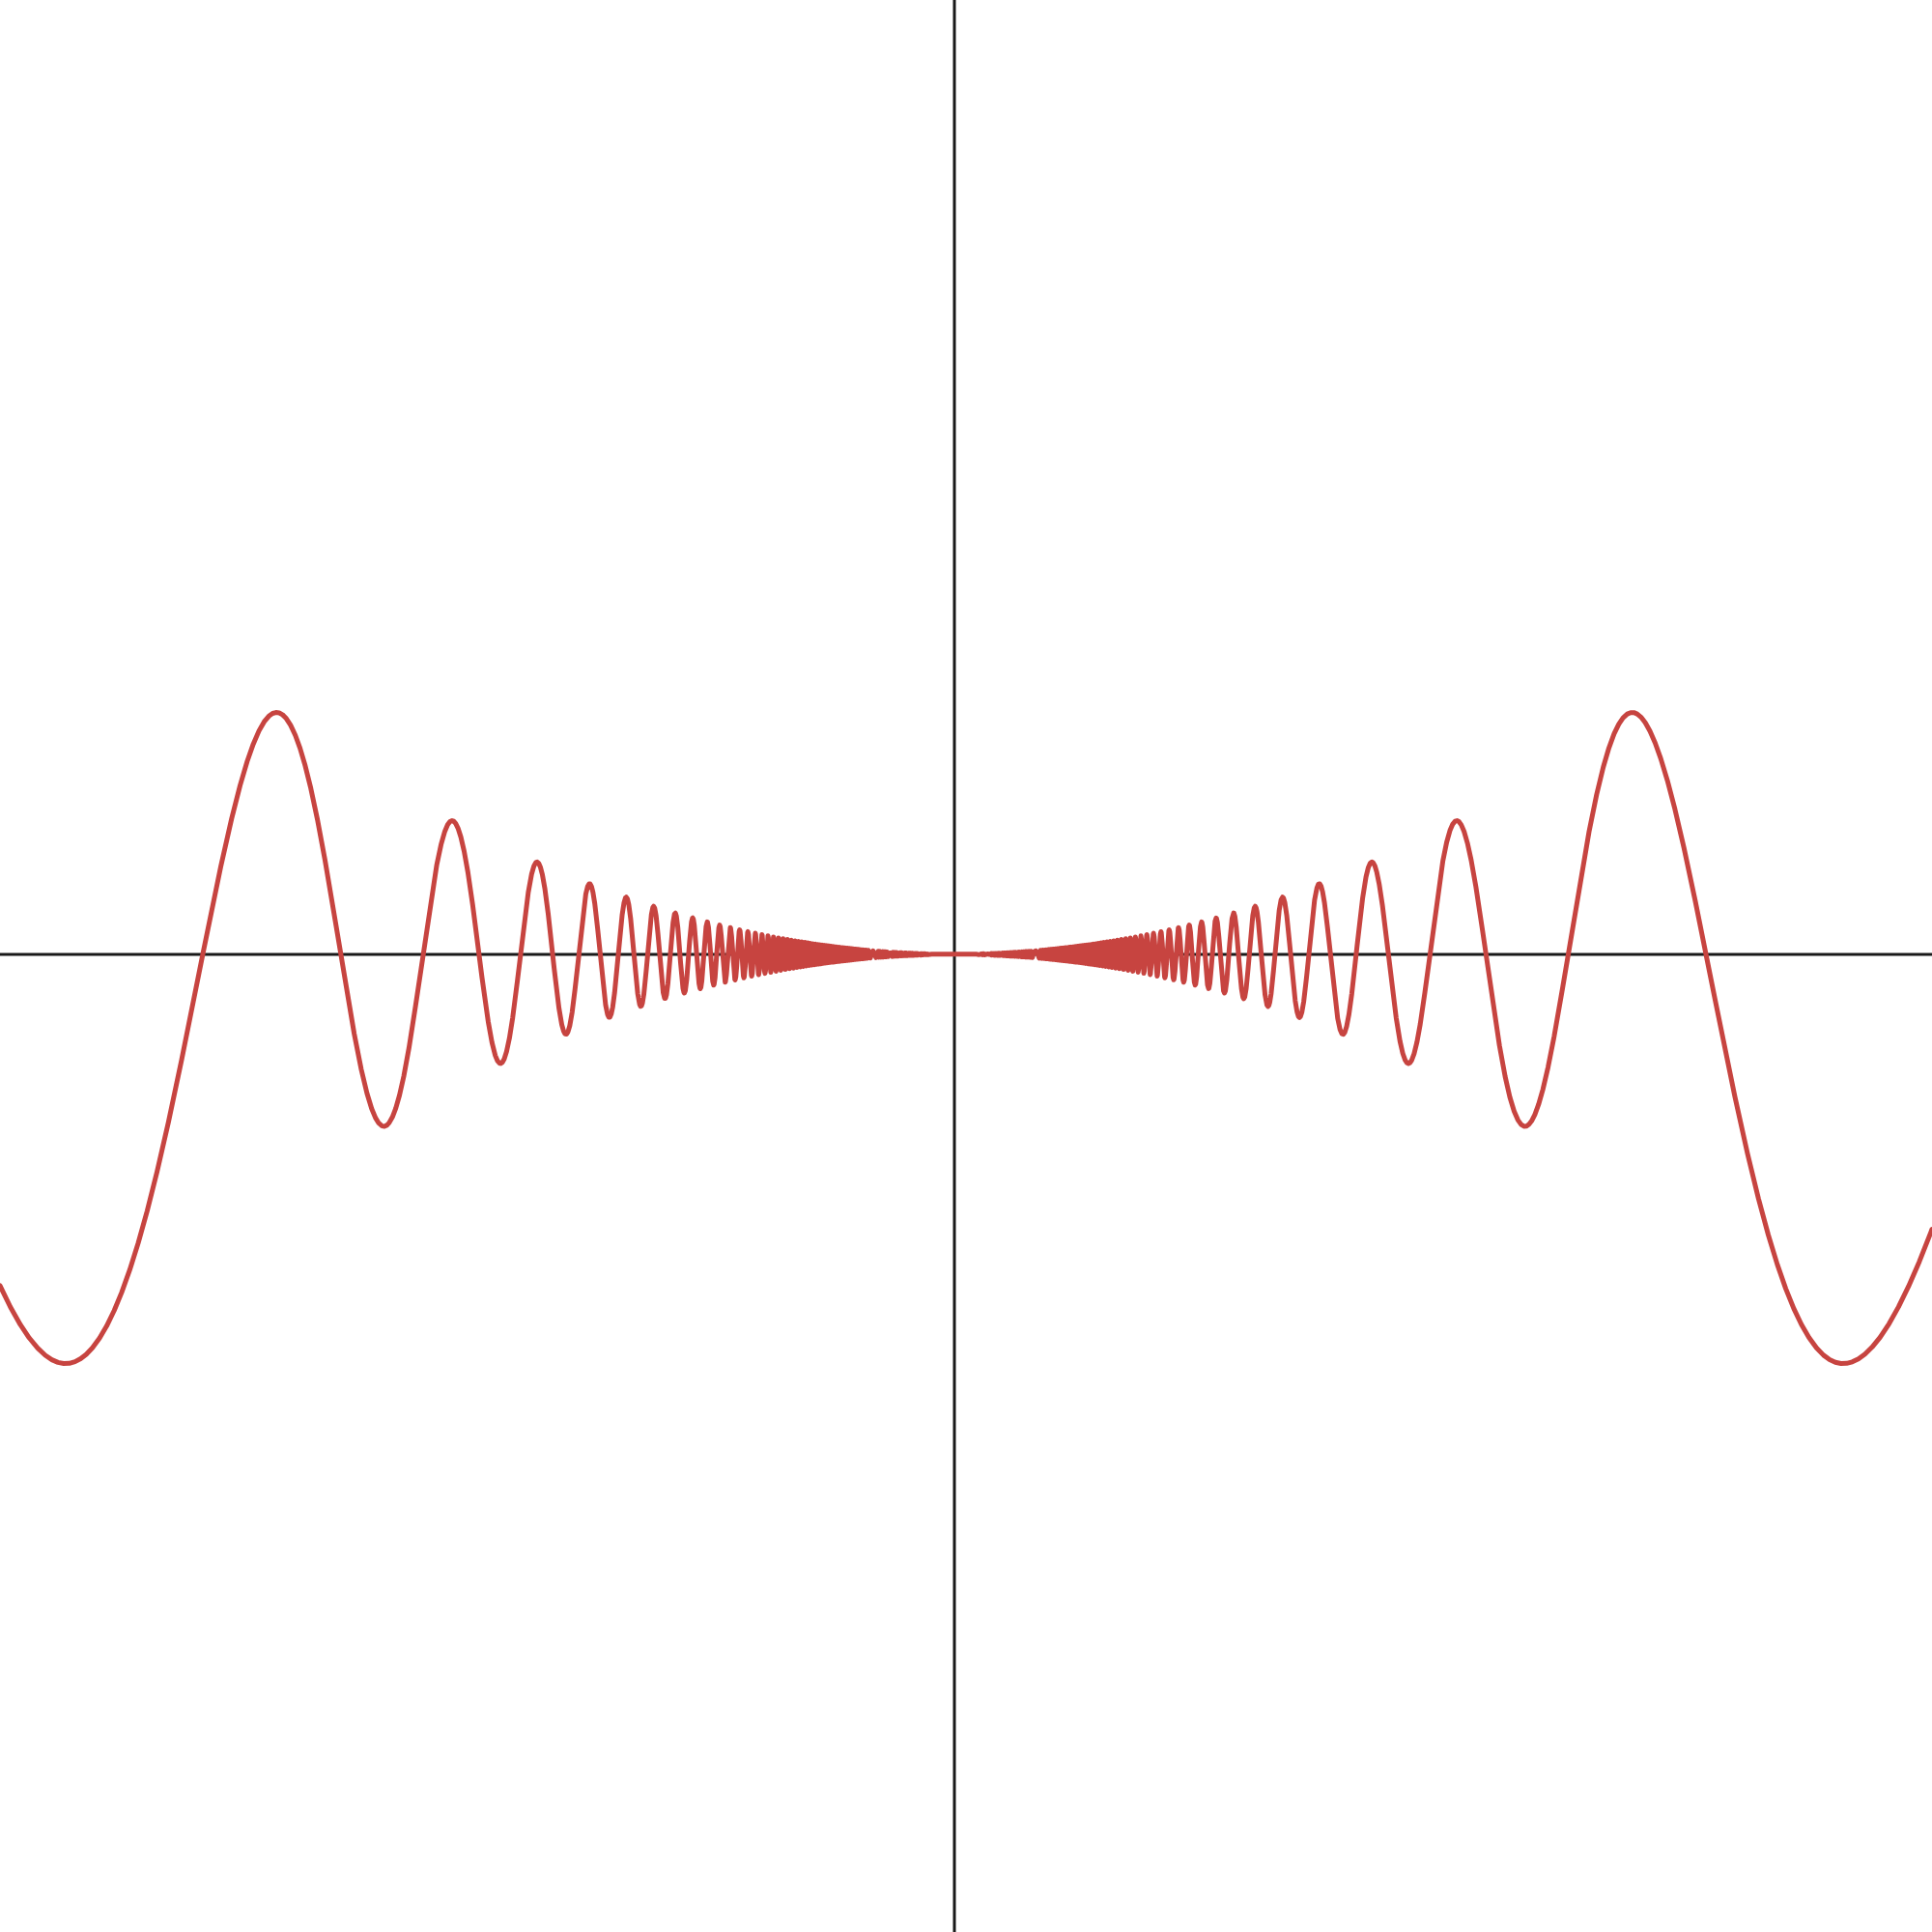
\includegraphics[width=1\linewidth]{Pictures/Fancy_sinus_for_not_Riemann_integrable_example.png}

% \end{wrapfigure}

\[
f(x) = \begin{cases}
    F'(x), & x \neq 0 \\
    F'(0), & x = 0
\end{cases}\]

$F'(0) = \lim_{x\rightarrow 0} \frac{x^2 \sin\left(\frac{1}{x^2}\right)}{x}
= \lim_{x\rightarrow 0} x \sin \frac{1}{x^2} = 0$

$F'(x) = 2x\cdot \sin \frac{1}{x^2} + x^2 \cos \frac{1}{x^2}\cdot
\left(\frac{-2}{x^2}\right) =
2x \sin\frac{1}{x^2} - \frac{2}{x}\cos \frac{1}{x^2}$
-- неограниченна на любом отрезке, содержащем 0

$\implies f \notin R([a, b])$, но $\exists$ первообразная $F$
\bigskip

Теперь приведём пример функции из (2). Здесь всё ещё проще:
нужно вспомнить, какие функции заведомом не имеют первообразной
-- те, которые имеют разрыв первого рода, так как производная
не может иметь разрыв первого рода, это следствие из теоремы Лагранжа о среднем.
Поэтому здесь простейший пример такой:

\[
f(x) = \begin{cases}
    1, & x > 0 \\
    0, & x = 0 \\
    -1, & x < 0
\end{cases}
\]
Это так называемый ''сигнум x'', $\mathrm{sgn}(x)$

$f \in \Rim([-1, 1])$ по критерию Лебега.
При этом первообразной нет, докажем это
\begin{proof}    
    \[\begin{aligned}
        \text{Предположим, что }\exists F\in \DIF([-1, 1]):\;
        F'(x) = f(x)\quad \forall x \in [-1, 1] \\
        \left.\begin{aligned}
        & \implies F'(x) = 1 \quad \forall x > 0 \implies
        \exists \lim_{x \rightarrow 0+0} F'(x) = 1 \implies
        \exists F'_+(0) = 1 \\
        & \implies F'(x) = -1 \quad \forall x < 0 \implies
        \exists \lim_{x\rightarrow 0-0} F'(x) = -1 \implies
        \exists F'_-(0) = -1
        \end{aligned}
        \right\} \implies \\
        \implies F'_+(0) \neq F'_-(0) \implies \nexists F'(0)
    \end{aligned}\]
    
    Получили противоречие с тем, что $F$ дифференцируема на всём отрезке $[-1, -1]$
\end{proof}

\begin{lemma}
    Пусть $f \in R([a, b])$. Тогда $F(x) = \int_a^x f(t) dt$ является
    непрерывной функцией от $x$
\end{lemma}
\begin{proof}
    $|F(x_1) - F(x_2)| \leqslant \left|\int_{x_1}^{x_2} f(t)dt\right|$,
    но $f$ -- ограничена $\implies |f(x)| \leqslant M \;
    \forall x \in [a, b]$

    $\implies \left|\int_{x_1}^{x_2} f(t)dt\right|
    \leqslant M|x_1 - x_2|$

    $\implies F$ -- равномерно непрерывна на $[a, b]$ 
\end{proof}

\begin{theorem}
    Пусть $f \in C([a, b])$. Тогда $F(x) = \int_a^x f(t) dt$
    непрерывно дифференцируема на $[a, b]$ и справедливо равенство
    $F'(x) = f(x)\quad \forall x \in [a, b]$. (с соответствующим
    соглашением в точках $a$ и $b$)
\end{theorem}
\begin{note}
    $\int_a^x f(t)dt$ называется интегралом с переменным
    верхним пределом
\end{note}
\begin{proof}
    Фиксируем точку $x^0 \in [a, b]$.

    $\left|\frac{F(x) - F(x^0)}{x - x^0} - f(x^0)\right|
    = \left|\frac{\int_{x^0}^x f(t)dt}{x - x^0} - f(x^0)\right|
    = \left|\frac{\int_{x^0}^x f(t)dt - \int_{x^0}^x f(x^0)dt}{x - x^0}\right|
    \leqslant \frac{\int_{x^0}^x |f(t) - f(x^0)|dt}{x - x^0}$

    Далее считаем $x > x^0$

    Но $f$ непрерывна в точке $x^0 \implies
    \forall \epsilon > 0\; \exists \delta(\epsilon) > 0:\;
    \forall x \in U_\delta^\circ(x^0) \cap [a, b]
    \hookrightarrow |f(x) - f(x^0)| < \epsilon$

    $\implies \forall x \in U_\delta^\circ(x^0) \hookrightarrow
    \frac{\int_{x^0}^x |f(t) - f(x^0)|dt}{x - x^0}
    < \frac{\epsilon \int_{x^0}^x dt}{x - x^0} = \epsilon$

    В итоге, $\forall \epsilon > 0 \exists \delta(\epsilon) > 0:\;
    \forall x \in U_\delta^\circ(x^0) \cap [a, b]
    \hookrightarrow \left|\frac{F(x) - F(x^0)}{x - x^0} - f(x^0)\right|
    < \epsilon$
\end{proof}
